% Generator: hand-authored TikZ schematic traced from the fixed source-visible tetrahedron edges; projection is illustrative.
% Source ID: src-96ac0e772a0483bbf7cf803b94b1a1d8d8e1d2ae16b936b196e6abc05d1251ee
% PDF SHA-256: 7e840dc5c259cf05138337178794a58b6593dc7f2bf0d693826489856da416e9
% PDF page 2; question 14.
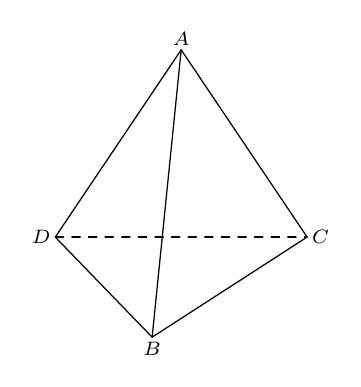
\begin{tikzpicture}[
  x=0.82cm,y=0.82cm,line width=0.45pt,line cap=round,line join=round,
  every node/.style={font=\scriptsize,inner sep=1.5pt}
]
  \coordinate (A) at (0,2.9);
  \coordinate (D) at (-1.95,0);
  \coordinate (C) at (1.95,0);
  \coordinate (B) at (-0.45,-1.55);

  % DC is the only hidden edge in the source.
  \draw[dashed] (D)--(C);
  \draw (A)--(D)--(B)--(C)--(A);
  \draw (A)--(B);

  \node[above] at (A) {$A$};
  \node[left] at (D) {$D$};
  \node[right] at (C) {$C$};
  \node[below] at (B) {$B$};
\end{tikzpicture}
